\documentclass[
	% -- opções da classe memoir --
	12pt,		% tamanho da fonte
	%openright,	% capítulos começam em pág ímpar (insere página vazia caso preciso)
	oneside,	% para impressão em verso e anverso. Oposto a oneside
	a4paper,	% tamanho do papel.
	% -- opções da classe abntex2 --
	chapter=TITLE,		% títulos de capítulos convertidos em letras maiúsculas
	%section=TITLE,		% títulos de seções convertidos em letras maiúsculas
	%subsection=TITLE,	% títulos de subseções convertidos em letras maiúsculas
	%subsubsection=TITLE,% títulos de subsubseções convertidos em letras maiúsculas
	% -- opções do pacote babel --
	english,	% idioma adicional para hifenização
	brazil		% o último idioma é o principal do documento
]{abntex2}



%----------------------------------------------------------------------------------------
% Definição dos Packages
%----------------------------------------------------------------------------------------

\usepackage{silence}                            % Pra pular erros bestas do glossario
\WarningFilter{glossaries}{Overriding \printglossary}
\WarningFilter{glossaries}{Overriding `theglossary'}

\usepackage[subentrycounter,seeautonumberlist,nonumberlist=true]{glossaries}
\usepackage[T1]{fontenc}	                    % Selecao de codigos de fonte. Afeta separação de sílabas
\usepackage[brazilian,hyperpageref]{backref}    % Paginas com as citações na bibl
\usepackage[alf]{abntex2cite}                   % Citações padrão ABNT
\usepackage{lastpage}		                    % Usado pela ficha catalografica
\usepackage{indentfirst}	                    % Indenta o primeiro paragrafo de cada seção
\usepackage{microtype} 		                    % Para melhorias de justificação
\usepackage{bibentry}   	                    % para inserir refs. bib. no meio do texto
\usepackage{listings}                           % Define as listas (numeradas)
\usepackage{tikzsymbols}                        % Simbolos matemáticos (usado pra colocar o logo)
\usepackage{textcomp, gensymb}                  % Pra poder usar o º (\degree)
\usepackage{fontspec}                           % Pacote para a fonte Arial
%\usepackage{helvet}                             % Usado para definir a fonte em Helvetica
%\usepackage[utf8]{inputenc}	                 % Codificacao do documento (conversão automática dos acentos)

%----------------------------------------------------------------------------------------
% Execução dos Packages
%----------------------------------------------------------------------------------------
\citebrackets{[}{]}
\setmainfont{Arial} % Define a fonte em Arial
%\renewcommand{\familydefault}{\sfdefault}       % Define em Helvetica

\makeindex                                      % compila o indice

\usepackage{color}

\definecolor{keywordstyle}{RGB}{0,0,255}
\definecolor{stringstyle}{RGB}{184,21,21}
\definecolor{commentstyle}{RGB}{0,128,0}

\lstset{
	basicstyle=\ttfamily\tiny,
	keywordstyle=\color{keywordstyle},
	stringstyle=\ttfamily\color{stringstyle},
	commentstyle=\color{commentstyle},
	backgroundcolor=\color{gray!5},
	extendedchars=true,
	breaklines=true,
	frame=tb,
	showstringspaces=false,
	numbers=left,
	numberstyle=\tiny
}
% Configurações do pacote backref
\renewcommand{\backrefpagesname}{Citado na(s) página(s):~}
\renewcommand{\backref}{}                       % Texto padrão antes do número das páginas
\renewcommand*{\backrefalt}[4]{                 % Define os textos da citação
	\ifcase #1

	\or
		Citado na página #2.
	\else
		Citado #1 vezes nas páginas #2.
	\fi}

% Espaçamentos entre linhas e parágrafos
\linespread{1.5}                                % Espaçamento da linha
\setlength{\parindent}{1.3cm}                   % O tamanho do parágrafo
\setlength{\parskip}{0.2cm}                     % Controle do espaçamento entre um parágrafo e outro

\makeglossaries
% ----------------------------------------------
% Entradas do Glossário
% ----------------------------------------------
\newglossaryentry{BD}
    {
    name={Banco de dados},
    description={Bancos de dados ou bases de dados são conjuntos de arquivos relacionados entre si com registros sobre pessoas, lugares ou coisas. São coleções organizadas de dados que se relacionam de forma a criar algum sentido e dar mais eficiência durante uma pesquisa ou estudo científico} 
    }

\newglossaryentry{Encriptar}
    {
    name={Encriptar},
    description={Em criptografia, encriptação, ou cifragem, é o processo de transformar informação usando um algoritmo de modo a impossibilitar a sua leitura a todos excepto aqueles que possuam uma identificação particular, geralmente referida como chave} 
    }

\newglossaryentry{IBM}
    {
    name={International Business Machines (IBM)},
    description={International Business Machines (IBM): A International Business Machines Corporation é uma empresa dos Estados Unidos voltada para a área de informática. A empresa é uma das poucas na área de tecnologia da informação com uma história
contínua que remonta ao século XIX} 
    }

\newglossaryentry{Key}
    {
    name={Key},
    description={Uma chave é um pedaço de informação que controla a operação de um algoritmo de criptografia. Na codificação, uma chave específica a transformação do texto puro em texto cifrado, ou vice-versa, durante a decodificação} 
    }

\newglossaryentry{LP}
    {
    name={Linguagem de Programação},
    description={A linguagem de programação é um método padronizado, formado por um conjunto de regras sintáticas e semânticas, de implementação de um código fonte - que pode ser compilado e transformado em um programa de computador, ou usado como script interpretado - que informará instruções de processamento ao computador} 
    }
    
\newglossaryentry{Malware}
    {
    name={Malware},
    description={Um código malicioso, programa malicioso, software nocivo, software mal-intencionado ou software malicioso, é um programa de computador destinado a infiltrar-se em um sistema de computador alheio de forma ilícita, com o intuito de causar alguns danos, alterações ou roubo de informações} 
    }

\newglossaryentry{Pycharm}
    {
    name={Pycharm},
    description={PyCharm é um ambiente de desenvolvimento integrado usado em programação de computadores, especificamente para a linguagem Python. É desenvolvido pela empresa tcheca JetBrains} 
    }

\newglossaryentry{Pycryptodome}
    {
    name={Pycryptodome},
    description={O PyCryptodome é uma biblioteca em python que trata de implementações de algoritmos de criptografia} 
    }

\newglossaryentry{Python}
    {
    name={Python},
    description={Python é uma linguagem de programação de alto nível, interpretada, de script, imperativa, orientada a objetos, funcional, de tipagem dinâmica e forte. Foi lançada por Guido van Rossum em 1991} 
    }

\newglossaryentry{Feistel}
    {
    name={Feistel},
    description={A criptografia, uma cifra de Feistel é uma estrutura simétrica usada na construção de cifras de bloco, o nome é uma homenagem ao físico e criptógrafo alemão Horst Feistel, que foi o pioneiro na pesquisa enquanto trabalhava na IBM; esta cifra é comumente conhecida como rede de Feistel} 
    }

\newglossaryentry{Software}
    {
    name={Software},
    description={Software, é um termo técnico que foi traduzido para a língua portuguesa como logiciário ou suporte lógico, é uma sequência de instruções a serem seguidas e/ou executadas, na manipulação, redirecionamento ou modificação de um dado ou acontecimento} 
    }

\newglossaryentry{SQLite}
    {
    name={SQLite},
    description={SQLite é uma biblioteca em linguagem C que implementa um banco de dados SQL embutido. Programas que usam a biblioteca SQLite podem ter acesso a banco de dados SQL sem executar um processo SGBD separado} 
    }

\newglossaryentry{VSCode}
    {
    name={VSCode},
    description={O Visual Studio Code é um editor de código-fonte desenvolvido pela Microsoft para Windows, Linux e macOS. Ele inclui suporte para depuração, controle Git incorporado, realce de sintaxe, complementação inteligente de código, snippets e refatoração de código} 
    }
% ----------------------------------------------
% Configurações do glossário
\renewcommand*{\glsseeformat}[3][\seename]{\textit{#1}  
\glsseelist{#2}}
\begin{document}
% Seleciona o idioma do documento (conforme pacotes do babel)
%\selectlanguage{english}
\selectlanguage{brazil}

% Retira espaço extra obsoleto entre as frases.
\frenchspacing

\newpage

% ==============================================
% ELEMENTOS PRÉ-TEXTUAIS
% ==============================================
\pretextual

% ----------------------------------------------
% Capa
% ----------------------------------------------
%\imprimircapa
% Capa personalizada sem o uso de \imprimircapa
\begin{capa}
	\begin{center}
		\begin{minipage}{1\textwidth}
			\large\centering\makebox[\textwidth]{
\includegraphics[scale=1]{imagens/Logo UNIP.png}}
		\end{minipage}
	\end{center}
	\begin{center}
		\LARGE\textbf{UNIP -- UNIVERSIDADE PAULISTA\\}
		\LARGE {Curso de Ciência da Computação}\\
		\vfill
		\ABNTEXchapterfont\Large\textbf{\MakeUppercase{ATIVIDADES PRÁTICAS SUPERVISIONADAS - APS}}
		\\\small{DESENVOLVIMENTO DE UMA FERRAMENTA PARA COMUNICAÇÃO EM REDE}
		\vfill
		\normalsize{
			André Ademir de Sousa Oliveira - N629630\\
			Daniel Chrispim Domingos - F263614\\
			Gabriel de Paula Seki - N6853H6\\
			Luiz Guilherme Davies Lencioni - N667125\\
			Marcos Vinicius Restani Avanzini - G13HJB9\\
			Vinícius Amorim - N641JC5\\
		}
		\vfill
		São José dos Campos, \today
	\end{center}
\end{capa}

% ----------------------------------------------
% Folha de rosto
% ----------------------------------------------
% folha de rosto personalizada sem uso de \imprimirfolhaderosto
\makeatletter
\renewcommand{\folhaderostocontent}{
	\begin{center}
		\begin{center}
			\begin{minipage}{1\textwidth}
				\large\centering\makebox[\textwidth]{
\includegraphics[scale=1]{imagens/Logo UNIP.png}}
			\end{minipage}
		\end{center}

		\vspace*{\fill}%\vspace*{\fill}
		\begin{center}
			\ABNTEXchapterfont\Large\textbf{\MakeUppercase{ATIVIDADES PRÁTICAS SUPERVISIONADAS - APS}}
			\\\small{DESENVOLVIMENTO DE UMA FERRAMENTA PARA COMUNICAÇÃO EM REDE}
		\end{center}
		\vspace*{\fill}

		\hspace{.45\textwidth}
		\begin{minipage}{.5\textwidth}
			\SingleSpacing
			{Atividades Práticas Supervisionadas do 5\degree\ Semestre do Curso de Ciência da Computação da \textbf{Universidade Paulista UNIP.}}
		\end{minipage}%
		\vspace*{\fill}


		\hspace{.45\textwidth}
		\begin{minipage}{.5\textwidth}
			{\textbf{Coordenador:} Prof. Fernando A. Gotti}%
		\end{minipage}%


		\hspace{.45\textwidth}
		\begin{minipage}{.5\textwidth}
			{\textbf{Prof. Responsável:} André Yoshimi Kusumoto}%
		\end{minipage}%


		\vspace*{\fill}
		%{\abntex@ifnotempty{\imprimirinstituicao}{\imprimirinstituicao\vspace*{\fill}}}

		São José dos Campos, \today
	\end{center}
}
\makeatother

% Folha de rosto (o * indica que haverá a ficha bibliográfica)

\imprimirfolhaderosto

% ||||||||||||||||||||||||||||||||||||||||||||||
% RESUMOS
% ||||||||||||||||||||||||||||||||||||||||||||||

% ----------------------------------------------
% Resumo em português
% ----------------------------------------------
% Importante: De acordo com a NBR6024 as palavras-chaves devem ser separadas entre si por ponto e devem ter somente a primeira palavra escrita com letra maiúscula
% \setlength{\absparsep}{18pt} % ajusta o espaçamento dos parágrafos do resumo
\begin{resumo}
	\text Este trabalho foi desenvolvido com o intuito de demonstrar a funcionalidade de uma aplicação de conversa através de uma rede, aplicando conceitos de comunicação em rede. Para este objetivo, foi apresentado uma introdução a diversos conceitos fundamentais ao entendimento da aplicação e transferência de dados através de uma rede.
	\text No decorrer deste documento, será detalhado as definições e padrões da Internet, os diferentes protocolos de comunicação e também os diferentes tipos de topologia de redes de comunicação.
	\vspace{\onelineskip}

	\noindent
	\textbf{Palavras-chaves}: Internet. Protocolos. Padrões da Internet. Redes. Topologia de Redes.
\end{resumo}

% ----------------------------------------------
% Resumo em inglês
% ----------------------------------------------
% Importante: De acordo com a NBR6024 as palavras-chaves devem ser separadas entre si por ponto e devem ter somente a primeira palavra escrita com letra maiúscula
\begin{resumo}[Abstract]
	\begin{otherlanguage*}{english}
		\text This document was developed within the intention of demonstrating the functionality of a local network chat application, applying concepts of network communication. To this objective, it was presented an introduction to various fundamental concepts to the understanding of the application and transfer of data through a network.
		\text Through this work, it will be detailed the definitions and standarts of the internet, the different protocols of communication aswell as many different kinds of communication network topologies.
		\vspace{\onelineskip}

		\noindent
		\textbf{Keywords}: Internet. Protocols. Internet Standarts. Networks. Network Topologies.
	\end{otherlanguage*}
\end{resumo}

% ----------------------------------------------
% inserir lista de ilustrações
% ----------------------------------------------
% \pdfbookmark[0]{\listfigurename}{lof}
% \listoffigures*
% \cleardoublepage

% Diferentes tipos de listas podem ser criadas por meio de macros do memoir.

% ----------------------------------------------
% inserir lista de tabelas
% ----------------------------------------------
% \pdfbookmark[0]{\listtablename}{lot}
% \listoftables*
% \cleardoublepage

% ----------------------------------------------
% inserir lista de abreviaturas e siglas
% ----------------------------------------------
% Importante: As abreviaturas e siglas devem estar em ordem alfabética
% \begin{siglas}
%   \item[ABNT] Associação Brasileira de Normas Técnicas
%   \item[abnTeX] ABsurdas Normas para TeX
% \end{siglas}

% ----------------------------------------------
% inserir lista de símbolos
% ----------------------------------------------
% Importante: Os símbolos devem estar na ordem de aparecimento no texto.
% \begin{simbolos}
%   \item[$ \Gamma $] Letra grega Gama
%   \item[$ \Lambda $] Lambda
%   \item[$ \zeta $] Letra grega minúscula zeta
%   \item[$ \in $] Pertence
% \end{simbolos}

% ----------------------------------------------
% inserir o sumário
% ----------------------------------------------
\pdfbookmark[0]{\contentsname}{toc}
\tableofcontents*
\cleardoublepage



%----------------------------------------------------------------------------------------
% Introdução, Objetivos e Justificativa
%----------------------------------------------------------------------------------------
\textual
\newpage\thispagestyle{empty}


\chapter{\textbf{Introdução}}

\par As redes de comunicações são intrínsecas à comunicação humana moderna. O conceito delas se manifesta de diversas formas no dia a dia, dos aplicativos de conversas, dos serviços de correio eletrônico à \textit{internet} em si. Até mesmo serviços essenciais à infraestrutura de cidades dependem dessas redes para realizarem suas funções. Por isso, o compreendimento do funcionamento dessas conexões, seus tipos e características individuais se torna cada vez mais importante conforme os avanços tecnológicos nesse meio se aceleram.

\par O conceito da comunicação entre dois ou mais computadores não é limitado apenas às \textit{chat rooms}, aos fóruns \textit{online} ou serviços de redes sociais. Toda transferência de dados é um tipo de comunicação e assim é aplicável a qualquer tipo de interação \textit{online} ou em uma rede física. Portanto, a importância do entendimento das definições e tecnologias que compõem essas interligações não pode ser reduzida.

\par Como uma conversa harmônica entre dois indivíduos, a comunicação entre computadores também segue uma série de regras que podem ser definidas como protocolos. Eles garantem que as informações enviadas e recebidas pelo remetente e destinatário sejam compreensíveis para o outro.
%----------------------------------------------------------------------------------------
\newpage\thispagestyle{empty}
\section{\textbf{Objetivos Gerais}}
\par Este trabalho busca apresentar os conceitos de redes de comunicação e comparar os diferentes métodos de implementação de uma rede física e o funcionamento de um programa que possibilita o envio de mensagens de texto através de uma conexão com interface gráfica.

\par Acredita-se que este documento possa demonstrar conhecimentos de diferentes métodos de desenvolvimento de \textit{software} de comunicação, além dos métodos existentes para se realizar as conexões necessárias para o funcionamento correto dos mesmos.

%----------------------------------------------------------------------------------------
\section{\textbf{Objetivos Específicos}}
\par Com o conhecimento apresentado durantes as aulas, estudos sobre comunicação entre computadores e a linguagem de programação \textit{Python}, foi desenvolvido um programa que utiliza uma conexão para transferir dados entre duas ou mais interfaces.

\par Além disso, foi disponibilizado exemplos de funções executadas no código e imagens detalhando os diferentes tipos de topologias, redes e protocolos potencialmente utilizados.
%----------------------------------------------------------------------------------------
\section{\textbf{Justificativa}}
\par Observando o funcionamento da aplicação criada para este trabalho, é perceptível o uso dos conceitos estudados durante o semestre, empenhando uma interface gráfica para simplificar o entendimento para um indivíduo leigo, sem conhecimento aprofundado de interfaces de linha de comando.


%----------------------------------------------------------------------------------------
% Tema Escolhido
%----------------------------------------------------------------------------------------
\newpage\thispagestyle{empty}
\chapter{\textbf{Fundamentos da Comunicação de Dados em Rede}}

\section{\textbf{Definição}}
\par Segundo (NOBREGA FILHO, 2016) “Rede é uma maneira de conectar computadores para que eles tenham consciência do outro e possam unir e compartilhar seus recursos”. Assim com a evolução da tecnologia e a grande necessidade de integrar um meio de comunicação entre os computadores e assim foi criado a comunicação de dados, essa criação permitiu que as máquinas conversem umas com as outras e assim facilitando diversas atividades.

\par Sua forma de funcionamento é através de um meio de transmissão físico, como cabos ou mais recentemente no ar \textit{Wi-Fi}, a informação transmitida é no formato binário \textit{bits} sendo a mais adequada já que as máquinas manipulam as informações em forma binária. (Porto Editora – redes de comunicação de dados na Infopédia, 2022).

%----------------------------------------------------------------------------------------
\newpage\thispagestyle{empty}
\section{\textbf{Internet}}
\par A sua origem foi em 1969 após uma necessidade de conectar os computadores dos departamentos da \textit{Advanced Research and Projects Agency} (\textit{ARPA}), assim gerou a \textit{ARPANET} que interligava quatro instituições: Universidade da Califórnia, LA e Santa Bárbara; Instituto de Pesquisa de Stanford e Universidade de Utah. (ESCOLA, Equipe Brasil. \textit{Internet}; Brasil Escola, 2022).

\par De acordo com o dicionário de Oxford \textit{Languages}, a \textit{Internet} é uma rede de computadores dispersos por todo o planeta que trocam dados e mensagens utilizando um protocolo comum, unindo usuários particulares, entidades de pesquisa, órgãos culturais, institutos militares, bibliotecas e empresas de toda envergadura”.

\par Com sua criação também surgiu a facilidade de transmitir dados para qualquer lugar do planeta e devido a recursos cada vez mais “pesados”, a velocidade de transmissão está cada vez mais necessária.


%----------------------------------------------------------------------------------------
\newpage\thispagestyle{empty}
\section{\textbf{Protocolos}}

\par Protocolo de rede é um conjunto de normas que permite às máquinas conectadas à internet se comuniquem entre si com uma linguagem universal, de forma que qualquer computador que seja produzido consiga interpretar o dado recebido ou enviado. (TEBALDI PEDRO, 2019)

\par Uma das funções dos protocolos de rede é coletar os dados transmitidos e dividir em pequenos pedaços que são denominados como pacotes, o pacote tem em si a informação do endereçamento de destino e origem do dado. (LONGEN ANDREI, 2018)

%----------------------------------------------------------------------------------------
\subsection{\textbf{IP}}

\par O protocolo \textit{IP} \textit{Internet Protocol} é um dos mais importantes na \textit{web}, com ele é possível fazer a elaboração e transmissão dos pacotes de dados, porém, a entrega dos pacotes não é garantida.

\par Com o endereço de IP (endereço da máquina) é possível determinar o destino da mensagem, então com a máscara de sub rede irá definir o endereço que se refere a rede de destino, e o campo de \textit{gateway} estreita por padrão saberá o computador específico. (LONGEN ANDREI, 2018)

%----------------------------------------------------------------------------------------
\newpage\thispagestyle{empty}
\subsection{\textbf{TCP/IP}}

\par \textit{TCP/IP} é o acrônimo da combinação de dois protocolos: o \textit{TCP} (\textit{Transmission Control Protocol}) e \textit{IP} (\textit{Internet Protocol}), essa combinação é responsável pelo envio e recebimento de dados por toda a internet.

\par A sua origem foi devido a diversas aplicações da \textit{ARPANET} referente à pesquisas militares em 1969, sua ideia é oferecer rápida troca de dados entre computadores conectados a uma rede. (TEBALDI PEDRO, 2019)

%----------------------------------------------------------------------------------------
\subsection{\textbf{HTTP/HTTPS}}

\par O protocolo \textit{HTTP} (\textit{Hypertext Transfer Protocol}) é utilizado para fazer a conexão entre cliente (\textit{browser}) e servidor (\textit{site}), ele é responsável em garantir a sua navegação em sites da internet. (TEBALDI PEDRO, 2019)

\par Seu funcionamento é baseado em um navegador que faz um pedido de acesso a uma página da web, e o servidor do site decide a permissão de acesso, nesse momento também é enviado os arquivos da página que o usuário deseja acessar. (TEBALDI PEDRO, 2019)

\par Já o\textit{ HTTPS} (\textit{Hyper Text Transfer Secure}) é uma camada extra de proteção que indica para o usuário quais sites são seguros para o acesso, para o site utilizar desse protocolo é necessário possuir um certificado \textit{SSL} que cria uma proteção entre o cliente e o servidor. Essa proteção é feita com uma criptografia que impede atividades maliciosas de coletar dados do usuário.

%----------------------------------------------------------------------------------------
\newpage\thispagestyle{empty}
\subsection{\textbf{FTP/SFTP}}

\par \textit{FTP} (\textit{File Transfer Protocol}) é um protocolo de transferência de dados mais simples entre duas máquinas pela rede.

\par Seu funcionamento é da seguinte forma. Um computador (cliente) faz um pedido de conexão com o servidor para pegar um documento ou arquivo, então o servidor recebe seu pedido de conexão e fornece ou não o arquivo para o cliente. (TEBALDI PEDRO, 2019)

\par Já o \textit{SFTP} (\textit{Simples File Transfer Protocol}) utiliza uma camada de proteção conhecida como \textit{SSH} (\textit{Secure Shell}) para autenticar e proteger a conexão entre cliente e servidor. No\textit{ SFTP} a transferência é feita por pacotes \textit{SSH}, assim o cliente pode definir a quantidade de arquivos que quer transferir e simultaneamente o sistema faz a criação das senhas para reforçar a segurança do processo. (TEBALDI PEDRO, 2019)

%----------------------------------------------------------------------------------------
\subsection{\textbf{Outros protocolos}}

\par Segue abaixo uma rápida abordagem de alguns outros tipos de protocolos e suas funções:

\par \textbf{Protocolo \textit{POP3} (\textit{Post Office Protocol 3}):} é um protocolo usado como mensagem eletrônica;

\par \textbf{Protocolo \textit{SSH} (\textit{Secure Shell}):} protocolo responsável pela proteção da troca de arquivos entre cliente e servidor;

\par \textbf{Protocolo \textit{SMTP} (\textit{Simple Mail Transfer Protocol}):} é conhecido por fazer o envio de mensagens eletrônicas, também conhecido como e-mails;

\par \textbf{Protocolo \textit{IMAP} (\textit{Internet Message Access Protocol}):} voltado para receber e enviar \textit{e-mails}, a sua diferença dos anteriores é a permissão do gerenciamento de arquivos e mensagens pelo usuário diretamente do próprio servidor.

%----------------------------------------------------------------------------------------
\newpage\thispagestyle{empty}
\section{\textbf{OSI}}

\par O modelo \textit{OSI} (\textit{Open System Interconnection}) foi lançado em 1984 e seu objetivo foi servir como modelo padrão para protocolos de comunicação entre diversos sistemas, sua arquitetura é dividida em 7 redes de computadores e o seu padrão permite que diferentes tecnologias sejam utilizadas em conjunto em um ambiente heterogêneo. (Nunes, 2020)

\par As camadas que compõem o modelo \textit{OSI} são as seguintes: aplicação, apresentação, sessão, transporte, rede, dados e física. (Nunes, 2020)

\begin{figure}[htbp]
	\centering
	\caption{Representação do Modelo OSI}
	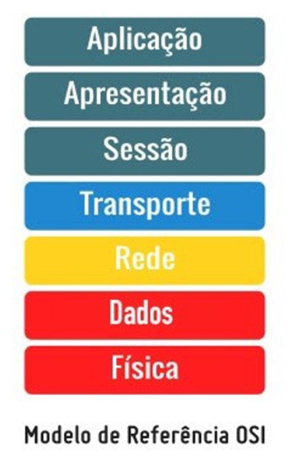
\includegraphics[]{imagens/modelo-osi.png}
	{\\Fonte: DataRain, 2020.}
	\label{fig:criação_1}
\end{figure}
%----------------------------------------------------------------------------------------
\newpage\thispagestyle{empty}
\section{\textbf{Redes}}

\par Em 1969 nos Estados Unidos, dava-se início a origem da internet, na época, era chamada de \textit{Arpanet} e tinha como únicos objetivos conectar universidades americanas e uso militar. Hoje, mais de cinco décadas depois, a Internet e as Redes de Computadores evoluíram explosivamente, tornando-se uma parte essencial da comunicação humana e da infraestrutura como sociedade. Hoje, segundo a ONU, 63\% da população mundial tem acesso à internet.

\par No passado, com a introdução dos microcomputadores no cenário da informática, havia uma estrutura distribuída, na qual, diversos equipamentos e computadores processavam informações de formas isoladas, o que costumava acarretando em uma série de problemas, como a duplicação desnecessária de recursos de hardware e de software. Foi neste cenário onde surgiu a criação das redes de computadores, introduzindo um sistema de comunicação entre as máquinas, permitindo o compartilhamento de recursos.  Uma rede pode ser definida como  um grupo de pelo menos dois computadores que estão ligados entre si, comunicando-se uns com os outros, compartilhando recursos e informações, com velocidade e praticidade.

%----------------------------------------------------------------------------------------
\newpage\thispagestyle{empty}
\subsection{\textbf{Taxonomia de Redes}}
\par As redes podem ser classificadas e divididas referentes a capacidade de alcance. São classificadas em:

\par \textbf{\textit{PAN – Personal Area Network}:} Comunicação direta entre dispositivos pessoais próximos, usados em residências e pequenos escritórios. Como exemplo \textit{smartwatches}, fones de ouvido sem fio, impressoras, caixas de som \textit{bluetooth}, entre outros dispositivos.

\par \textbf{\textit{LAN – Local Area Network}:} Redes privadas localizadas num mesmo prédio, sala ou campus, abrangendo alguns quilômetros de extensão. São utilizadas principalmente para o compartilhamento de recursos e troca de informações.

\par \textbf{\textit{MAN – Metropolitan Area Network}:} Semelhantes à \textit{LAN}, porém consegue abranger maiores áreas, como uma cidade inteira.

\par \textbf{\textit{WAN – Wide Area Network}:} Abrangem grandes áreas, como um país ou um continente inteiro.

%----------------------------------------------------------------------------------------
\newpage\thispagestyle{empty}
\subsection{\textbf{Topologias de Redes}}

\par Dá-se o nome de Topologia de Redes a disposição física que os computadores estão organizados, suas conexões lógicas. Tem-se as seguintes topologias:

\par \textbf{Topologia de Barramento:} Topologia onde todos os computadores estão interligados em um único cabo, com uma peça chamada de Terminador de Barramento em cada ponta. Cada nó na barra tem acesso às informações transmitidas. Esta característica facilita as aplicações com mensagens para múltiplas estações.

\begin{figure}[htbp]
	\centering
	\caption{Topologia Barramento}
	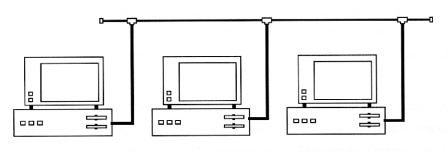
\includegraphics[]{imagens/topologia-barramento.png}
	{\\Fonte: Souza, 2009.}
	\label{fig:criação_1}
\end{figure}

\textbf{Vantagens:}\\
• Facilidade na instalação;\\
• Baixo custo;\\
• Baixa necessidade de cabos.\\

\textbf{Desvantagens:}\\
• Dificuldade em descobrir a causa de problemas de transmissão;\\
• Se o cabo se danificar a rede deixará de funcionar;\\
• A rede se torna mais lenta com uso intenso;\\
• Excesso de colisões.\\


\newpage\thispagestyle{empty}
\par \textbf{Topologia Estrela:} Nesta topologia, cada nó é interligado em um nó central (chamado de mestre), que é o centro de controle, comumente sendo um \textit{HUB} ou um concentrador. Topologia Estrela é comum em ambientes de rede de grande porte.

\begin{figure}[htbp]
	\centering
	\caption{Topologia Estrela}
	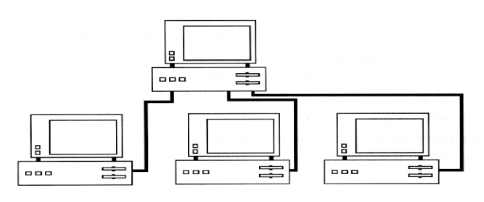
\includegraphics[]{imagens/topologia-estrela.png}
	{\\Fonte: Souza, 2009.}
	\label{fig:criação_1}
\end{figure}

\textbf{Vantagens:}\\
• Gerenciamento Centralizado;\\
• A adição de estações pode ser feita conectando-se às portas de comunicação que estejam livres;\\
• A análise de problemas na rede é mais simples;\\
• Uma máquina ou cabo defeituoso não afeta o funcionamento da rede.\\


\textbf{Desvantagens:}\\
• O número de estações fica limitado ao número de portas do \textit{HUB} ou do \textit{Switch};\\
• Maior quantidade de cabos;\\
• Custo elevado.\\


\newpage\thispagestyle{empty}
\par \textbf{Topologia Anel:} Nesta topologia, os computadores são todos conectados em forma de \textit{loop} fechado. Um cabo conecta o primeiro computador ao segundo, o segundo ao terceiro e assim por diante, até que o último computador se conecte ao primeiro, formando um círculo (logicamente, fisicamente não há necessidade de formar um círculo). Na Topologia Anel a Informação circula unidirecionalmente até voltar ao remetente.

\begin{figure}[htbp]
	\centering
	\caption{Topologia Anel}
	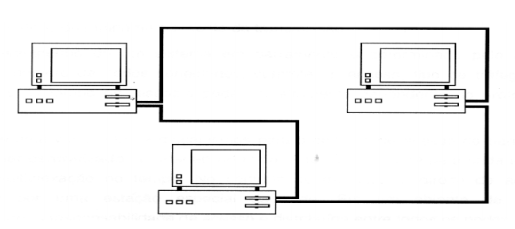
\includegraphics[]{imagens/topologia-anel.png}
	{\\Fonte: Souza, 2009.}
	\label{fig:criação_1}
\end{figure}

\textbf{Vantagens:}\\
• Facilidade na adição e remoção de estações;\\
• Pouca tolerância a falhas.\\


\textbf{Desvantagens:}\\
• Mais cara;\\
• Complexidade de instalação;\\
• Se um nó sair do ar, todo o sistema fica indisponível.\\


%----------------------------------------------------------------------------------------
\newpage\thispagestyle{empty}
\section{\textbf{Sinais e Transmissão}}
\par A camada física tem como função possibilitar a transmissão de uma sequência de \textit{Bits} pela rede, função esta que se dá na conversão destes \textit{Bits} em sinais eletromagnéticos. Em resumo, a conversão de sinais para a transmissão consiste em modificar o sinal contendo a informação e transmiti-la com a menor distorção possível, em uma faixa de frequência limitada, com facilidade de recuperação da informação na recepção e com o menor custo possível.

\par Na camada física, vários problemas podem acontecer afetando a transmissão do sinal, entre eles:
\par \textbf{Atenuação:} Acontece quando um sinal viaja por um meio físico, perdendo parte da sua energia para superar a resistência deste meio físico. É assim que um fio transportando sinais elétricos ganha um aumento de temperatura (ficando morno ou até mesmo quente), já que uma parte da energia elétrica do sinal é convertida em calor. Para resolver este problema, é necessário a utilização de amplificadores para aumentar o sinal.

\par \textbf{Distorção:} Cada componente do sinal apresenta uma velocidade de propagação em um meio e um certo atraso até chegar ao destino. Estas diferenças no atraso podem criar uma diferença de fase se o valor do atraso não for igual à duração do período, e a este problema é dado o nome de distorção de sinais.

\par \textbf{Ruído:} Ruídos são fatores externos que acabam corrompendo os sinais, diversos tipos de ruídos podem ser prejudiciais, como:\\
• \textbf{Ruído Térmico} - consiste no movimento aleatório de elétrons em um fio, o qual gera um sinal extra não enviado originalmente pelo emissor;\\
• \textbf{Ruído Indutivo} - provém de fontes como motores e eletrodomésticos;\\
• \textbf{Diafonia} - corresponde ao efeito de um fio sobre o outro;\\
• \textbf{Ruído Impulsivo} - um sinal com energia elevada e duração muito curta proveniente de linhas de transmissão de energia.\\



%----------------------------------------------------------------------------------------
% Estrutura do Software
%----------------------------------------------------------------------------------------
\newpage\thispagestyle{empty}
\chapter{\textbf{Plano de Desenvolvimento da Aplicação}}

\par

\begin{figure}[htbp]
	\centering
	\caption{Importação de Modulos no Server.py}
	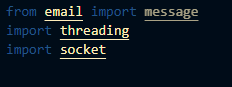
\includegraphics[]{PrintsServer/Captura de tela 2022-05-01 164434.png}
	{\\Fonte: Autoria Própria, 2022.}
	\label{fig:criação_1}
\end{figure}

\par No começo do código foi feita a importação dos módulos de \textit{message}, \textit{threading} e \textit{socket} que serão utilizados.
\newline

\begin{figure}[htbp]
	\centering
	\caption{Definição de Host e Porta no Server.py}
	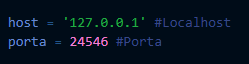
\includegraphics[]{PrintsServer/HostPort.png}
	{\\Fonte: Autoria Própria, 2022.}
	\label{fig:criação_1}
\end{figure}

\par No projeto foi utilizado o \textit{IP} do \textit{Local Host}, mas também é possível a utilização de um \textit{IP} de um servidor privado, a porta foi definida aleatoriamente do numero 5000 para cima, portas estas que o \textit{Windows} não usa por padrão.
\newline

\begin{figure}[htbp]
	\centering
	\caption{Listas de Clientes e Apelidos no Server.py}
	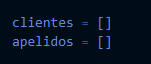
\includegraphics[]{PrintsServer/Client.png}
	{\\Fonte: Autoria Própria, 2022.}
	\label{fig:criação_1}
\end{figure}

\par Foram usadas listas vazias para, posteriormente, acrescentar via código os nomes e os Clientes que serão definidos.
\newline

\newpage\thispagestyle{empty}
\begin{figure}[htbp]
	\centering
	\caption{Definindo método Broadcast no Server.py}
	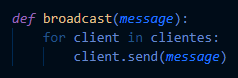
\includegraphics[]{PrintsServer/Broadcast.png}
	{\\Fonte: Autoria Própria, 2022.}
	\label{fig:criação_1}
\end{figure}

\par Esse método faz com que toda mensagem enviada por qualquer usuário seja replicada para todos os usuários.
\newline

\begin{figure}[htbp]
	\centering
	\caption{Definindo método handle no Server.py}
	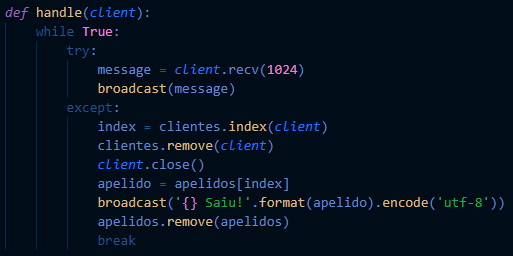
\includegraphics[]{PrintsServer/handle.png}
	{\\Fonte: Autoria Própria, 2022.}
	\label{fig:criação_1}
\end{figure}


\par O método \textit{handle} mantém o servidor aberto para receber novas mensagens e, caso algum usuário saia, ele mostra qual usuário é este.
\newline

\newpage\thispagestyle{empty}
\begin{figure}[htbp]
	\centering
	\caption{Definindo método Receber no Server.py}
	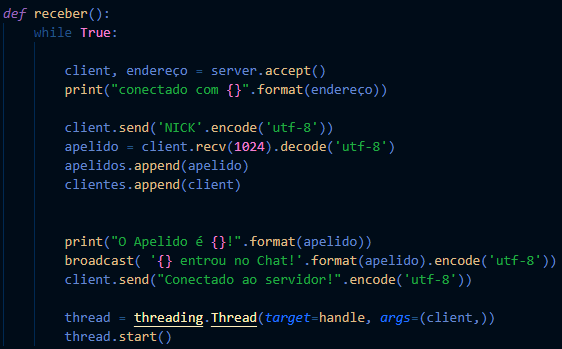
\includegraphics[]{PrintsServer/Receber.png}
	{\\Fonte: Autoria Própria, 2022.}
	\label{fig:criação_1}
\end{figure}

\par No método Receber o servidor vai receber o cliente e o endereço de \textit{IP} e aceitar ele como um novo usuário, depois faz com que ele defina o seu apelido e depois mostrar aos outros usuários quem entrou na sala de chat.
\newline

\begin{figure}[htbp]
	\centering
	\caption{Importação de módulos no client.py}
	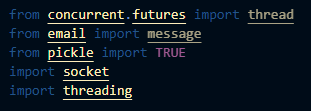
\includegraphics[]{PrintsServer/clientimport.png}
	{\\Fonte: Autoria Própria, 2022.}
	\label{fig:criação_1}
\end{figure}

\par No começo do código foi feita a importação dos módulos que serão usados mais tarde.
\newline
\newpage\thispagestyle{empty}
\begin{figure}[htbp]
	\centering
	\caption{Definição do apelido e qual o IP e porta vai conectar no client.py}
	\includegraphics[]{PrintsServer/CLientcomeço.png}
	{\\Fonte: Autoria Própria, 2022.}
	\label{fig:criação_1}
\end{figure}


\par Nesta parte do código é onde ocorre a definição do apelido do usuário e qual o \textit{IP} e Porta o Cliente ira conectar.
\newline

\begin{figure}[htbp]
	\centering
	\caption{Definindo o método receber no client.py}
	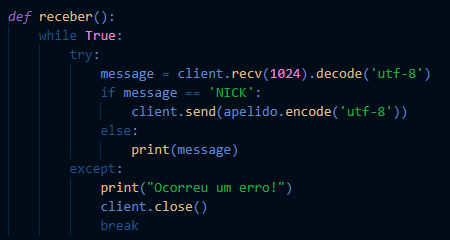
\includegraphics[]{PrintsServer/clientreceber.png}
	{\\Fonte: Autoria Própria, 2022.}
	\label{fig:criação_1}
\end{figure}

\par Este método é para o usuário receber a receber a mensagem de outros usuários que estão conectados no servidor, pode-se ver que se o Cliente receber a palavra 'NICK' irá mandar o apelido para o servidor, isso ocorre pois no método Receber do \textit{Server.py} ele envia uma mensagem escrita 'NICK' para chamar esse modulo, assim atribuindo o apelido do usuário a lista vazia.
\newline

\newpage\thispagestyle{empty}
\begin{figure}[htbp]
	\centering
	\caption{Definindo o método escrever no client.py}
	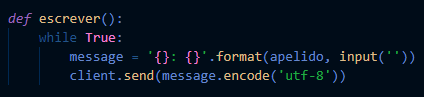
\includegraphics[]{PrintsServer/clientescrever.png}
	{\\Fonte: Autoria Própria, 2022.}
	\label{fig:criação_1}
\end{figure}

\par Este método é usado para pegar o \textit{Input} do usuário e manda-lo para o servidor que depois irá replicar essa mensagem para todos pelo método \textit{Broadcast}.
\newline

\begin{figure}[htbp]
	\centering
	\caption{Servidor funcionando}
	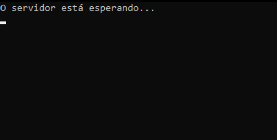
\includegraphics[]{Printis/Servidorlistening.png}
	{\\Fonte: Autoria Própria, 2022.}
	\label{fig:criação_1}
\end{figure}

\par Nesse passo o servidor esta esperando algum cliente se conectar com ele.

\newpage\thispagestyle{empty}
\begin{figure}[htbp]
	\centering
	\caption{Servidor com Clientes conectados}
	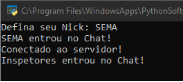
\includegraphics[]{Printis/Sema.png}
	{\\Fonte: Autoria Própria, 2022.}
	\label{fig:criação_1}
\end{figure}

\par Neste passo é onde já ocorreu a conexão dos usuários ao servidor pelo Cliente.

\begin{figure}[htbp]
	\centering
	\caption{Cliente definindo o apelido do usuário}
	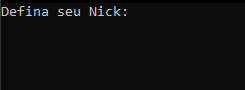
\includegraphics[]{PrintsServer/ClientNick.png}
	{\\Fonte: Autoria Própria, 2022.}
	\label{fig:criação_1}
\end{figure}

\par Neste passo define-se o nome do usuário para identificação do servidor.

\begin{figure}[htbp]
	\centering
	\caption{Cliente}
	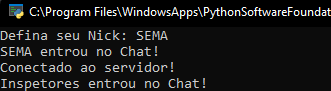
\includegraphics[]{Printis/ClientCOn.png}
	{\\Fonte: Autoria Própria, 2022.}
	\label{fig:criação_1}
\end{figure}

\par Agora o cliente mostra quem acabou de entrar no seu chat e mostra que você esta conectado no servidor.
\newpage\thispagestyle{empty}
\begin{figure}[htbp]
	\centering
	\caption{Mandar a mensagem}
	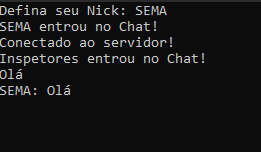
\includegraphics[]{Printis/ClientMandarMSg.png}
	{\\Fonte: Autoria Própria, 2022.}
	\label{fig:criação_1}
\end{figure}

\par Neste passo o usuário esta escrevendo sua mensagem que sera replicada pelo servidor para o outro usuário

\begin{figure}[htbp]
	\centering
	\caption{Receber a Mensagem}
	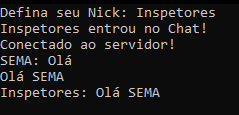
\includegraphics[]{Printis/OlaSema.png}
	{\\Fonte: Autoria Própria, 2022.}
	\label{fig:criação_1}
\end{figure}

\par Agora o usuário Inspetores recebeu a mensagem da SEMA e consegue responder a pergunta.
%----------------------------------------------------------------------------------------
% Código Fonte
%----------------------------------------------------------------------------------------
\newpage\thispagestyle{empty}
\chapter{\textbf{Relatório com as Linhas de Código}}
\renewcommand\lstlistingname{\textbf{Arquivo}}

\lstinputlisting[language=Python, label=Server, caption={Server.py}]{codigos/Server.py}

\newpage\thispagestyle{empty}
\lstinputlisting[language=Python, label=Client, caption={Client.py}]{codigos/client.py}
\newpage\thispagestyle{empty}

% ==============================================
% ELEMENTOS PÓS-TEXTUAIS
% ==============================================
\postextual

% ||||||||||||||||||||||||||||||||||||||||||||||
% REFERÊNCIAS BIBLIOGRÁFICAS
% ||||||||||||||||||||||||||||||||||||||||||||||
\nocite{{ref01}, {ref02}, {ref03}, {ref04}, {ref05}, {ref06}, {ref07}, {ref08}}
\nocite{{ref09}, {ref10}, {ref11}, {ref12}, {ref13},{ref14},{ref15}}

\bibliography{references}

% ==============================================
% INDICE REMISSIVO
% ==============================================
\phantompart
\printindex

% ----------------------------------------------------------
% Glossário
% ----------------------------------------------------------

% ---
% Define nome e preâmbulo do glossário
% ---
\phantompart
\renewcommand{\glossaryname}{GLOSSÁRIO}
% ---
% Estilo de glossário
% ---
% \glossarystyle{tree}
% \glossarystyle{altlisthypergroup}
\setglossarystyle{index}
\glsaddall

% ---
% Imprime o glossário
% ---
\cleardoublepage
\phantomsection
\addcontentsline{toc}{chapter}{\glossaryname}
% \printglossaries
% ---
\end{document}
